\documentclass[../../main.tex]{subfiles}
\begin{document}
\section{Teilerbeziehung und Ideale}

\begin{df}\label{16.1.1}
Wir führen auf $A$ die Relationen \emph{$\mid$}\index{Teilbarkeit@{\bf Teilbarkeit}!Teilbarkeitsrelation} und \emph{$\divi$}\index{Teilbarkeit@{\bf Teilbarkeit}!Assozitation} ein für durch
\begin{align*}
a\mid b:\Longleftrightarrow \exists c\in A: ac=b,\ (a,b\in A),
\end{align*}
gesprochen
\begin{itemize}
\item $''a\text{ \emph{teilt}\index{Teilbarkeit@{\bf Teilbarkeit}!Teiler} }b\text{ (in }A)''$
\item $''a\text{ ist Teiler von }b\text{ (in }A)''$
\item $''b\text{ ist Vielfaches von }a\text{ (in }A)''$ ,
\end{itemize}
sowie
\begin{align*}
a\divi b:\Longleftrightarrow (a\mid b\land b\mid a),\ (a,b\in A),
\end{align*}
gesprochen
\begin{itemize}
\item $''a\text{ ist assoziativ zu } b\text{ (in }A)''$
\item $''a\text{ und }b\text{ sind assoziativ (zueinander) (in}A)''$.
\end{itemize}
\end{df}
	
\begin{er}\mbox{}[$\to$ \ref{3.3.4}]\label{16.1.2} 
Eine Untergruppe $I$ der additiven Gruppe von $A$ heißt Ideal von $A$, wenn $\forall a\in A: \forall b\in I: ab\in I$ [$\to$\ref{3.3.4}]. Für $a\in A$ ist $(a):=\{ca\in A\}$ das kleinste Ideal $I$ von $A$ mit $a\in I$, genannt das von $a$ erzeugte (Haupt-)Ideal. Man nennt ein Ideal $I$ von $A$ ein Hauptideal, wenn es $a\in A$ gibt mit $I=(a)$ [$\to$\ref{3.3.11}].
\end{er}

\begin{bem}\label{16.1.3} 
Seien $a,b\in A$. Dann gilt $a\mid b\Longleftrightarrow b\in (a)\Longleftrightarrow (b)\subseteq (a)$ und $a\divi b\Longleftrightarrow (a)=(b)$
Insbesondere ist $\divi$ eine Äquivalenzrelation [$\to$\ref{1.3.1}(b)] auf $A$ und auf der Quotientenmenge [$\to$\ref{1.3.4}(a)] $A/\divi$ können wir eine Halbordnung [$\to$\ref{12.1.1}] $\preceq$ definieren durch
\begin{align*}
\tc a\preceq \tc b:\Longleftrightarrow a\mid b,\ (a,b\in A),
\end{align*}
wobei für jedes $a\in A$ mit $\tc a:=\stackrel{\divi}{a}$ die Äquivalenzklasse [$\to$\ref{1.3.1}(b),\ref{2.3.1}] von $a$ bezeichnet wird. In der Tat: Sind $a,a',b,b'\in A$ mit $\tc a=\tc{a'}$ und $\tc b=\tc{b'}$, so gilt, dass $(a)=(a')$ und $(b)=(b')$ und daher
\begin{align*}
a\mid b\Longleftrightarrow (b)\subseteq (a)\Longleftrightarrow (b')\subseteq (a')\Longleftrightarrow a'\mid b'.
\end{align*}
\end{bem}

\begin{df}\label{16.1.4} 
Sei $B\subseteq A$ und $a\in A$. Es heißt $a$ ein \case{\emph{gemeinsamer Teiler (gT)}\index{Teilbarkeit@{\bf Teilbarkeit}! gemeinsamer Teiler (gT)}}{\emph{gemeinsames Vielfaches (gV)}\index{Teilbarkeit@{\bf Teilbarkeit}! gemeinsames Vielfaches (gV)}} der Elemente von $B$ (in $A$), wenn $\tc a$ eine \case{obere}{untere} Schranke von $\{\tc b\mid b\in B\}$ in $(A/\divi, \preceq)$ ist. Es heißt $a$ ein \case{\emph{größten gemeinsamen Teiler (ggT)}\index{Teilbarkeit@{\bf Teilbarkeit}! größter gemeinsamer Teiler (ggT)}}{\emph{kleinsten gemeinsamen Vielfachen (kgV)}\index{Teilbarkeit@{\bf Teilbarkeit}! kleinstes gemeinsames Vielfaches (kgV)}} der Elemente von $B$, wenn $a$ \case{Supremum}{Infimum} von $\{\tc b\mid b\in B\}$ in $(A/\divi, \preceq)$ ist.
\end{df}
	
\begin{df}\label{16.1.5}
Seien $(A_1,\preceq_2)$ und $(A_2,\preceq_2)$ halbgeordnete Mengen. Eine Abbildung $f: A_1\to A_2$ heißt Isomorphismus halbgeordneter Mengen, wenn $f$ bijektiv ist und
\begin{align*}
\forall a,b\in A_1: (a\preceq_1 b\Longleftrightarrow f(a)\preceq_2 f(b)).
\end{align*}
\end{df}

\begin{bem}\label{16.1.16}
Sei $B\subseteq A$ und $a\in A$.
\begin{enumerate}[\normalfont(a)]
\item Es ist klar, wie man die Definition von gT, gV, ggT, kgV ohne die Verwendung von $\divi$ lesen kann:
\begin{itemize}
\item $\text{a gT der El. von B }\Longleftrightarrow \forall b\in B: a\mid b$
\item $\text{a ggT der El. von }B \Longleftrightarrow\begin{pmatrix*}[l]\text{a gT der El. von B}\land\\ \forall b\in A: (\text{b gT der El. von B}\implies b\mid a)\end{pmatrix*}$

\end{itemize}
\item Wegen der Eindeutigkeit von Infima und Suprema in halbgeordneten Mengen [$\to$\ref{12.1.6}] sind ggT und kgV in kommutativen Ringen genau bis auf Assoziiertheit eindeutig, sofern sie existieren.
\item Betrachte die durch Obermengeninklusion (umgekehrte Inklusion) halbgeordnete Menge aller Hauptideale $H:=\{(a)\mid a\in A\}$. Nach Definition von $\divi$ ist die Abbildung $A/\divi\to H, \hat{a}\mapsto (a)$ wohldefiniert und injektiv. Offenbar ist sie auch surjektiv. Nach Definition von $\preceq$ ist sie ein Isomorphismus halbgeordneter Mengen. In der Definition von gT/ gV/ ggT/ kgV [$\to$\ref{16.1.4}] könnte man daher genauso $(a)$ statt $\tc{a}$, $(b)$ statt $\tc{b}$ und $(H,\supseteq)$ statt $(A/\divi,\preceq)$ schreiben.
\end{enumerate}
\end{bem}

\begin{er}\label{16.1.17}
\begin{enumerate}[\normalfont(a)]
\item Die Schnittmenge einer Menge von Idealen in $A$ ist wieder ein Ideal von $A$ [$\to$\ref{3.3.8}].
\item Für jede Teilmenge $E\subseteq A$ gibt es ein kleinstes Ideal, welches $E$ enthält [$\to$\ref{3.3.9}]. Man nennt es das von $E$ erzeugte Ideal und notiert es mit $(E)=(E)_A$. Es besteht gerade aus allen Summen von Vielfachen von Elementen von $E$ [$\to$\ref{3.3.10}].
\end{enumerate}
\end{er}

\begin{pro}\label{16.1.8}
Sei $B\subseteq A$ und $a\in A$.
\begin{enumerate}[\normalfont(a)]
\item $a\text{ gT der El. von }B\Longleftrightarrow B\subseteq (a)\Longleftrightarrow(B)\subseteq (a)$
\item $a\text{ gV der El. von }B\Longleftrightarrow a\in\bigcap\{(b)\mid b\in B\}\Longleftrightarrow (a)\subseteq\bigcap\{(b)\mid b\in B\}$
\item $a\text{ ggT. der El. von }B\Longleftarrow (a)=(B)$\\
und wenn $(B)$ ein Hauptideal ist, gilt auch ''$\implies$''.
\item $a\text{ kgV. der El. von }B\Longleftrightarrow (a)=\bigcap\{(b)\mid b\in B\}$
\end{enumerate}
\end{pro}
\begin{cproof}
(a) und (b) sind klar.\\

\noindent\textbf{Zu (c)}. 
\begin{itemize}
\item[$\impliedby$] Gelte $(a)=(B)$. Nach (a) ist $a$ ein gT der Elemente von B. Sei $b$ ein gT der Elemente von B. Zu zeigen ist $b\mid a$. Dann $a\in (a)=(B)\stackrel{(a)}{\subseteq}(b)$ und daher $b\mid a$.
\item[$\implies$] Sei $a$ ein ggT. der Elemente von $B$ und $b\in A$ mit $(b)=(B)$. Nach (a) gilt $(B)\subseteq (a)$. Noch zu zeigen ist $(a)\subseteq (B)$. Da $b$ ein gT. und $a$ ein ggT. der Elemente von $B$ ist, gilt $b\mid a$, also $(a)\subseteq (b)=(B)$.\\
\end{itemize}
\noindent\textbf{Zu (d)}. Wegen $(b)$ genügt es zu zeigen
\begin{align*}
	(\forall c\in A:(\underbrace{c\text{ gV der El. von }B}_{\Longleftrightarrow c\in \bigcap\{(b)\mid b\in B\}}\implies a\mid c))\Longleftrightarrow (a)\supseteq\bigcap\{(b)\mid b\in B\}.
\end{align*}
Dies ist klar.
\end{cproof}

\begin{bem}\label{16.1.9}
In \ref{3.3.13} haben wir gezeigt, dass in $\Z$ jedes Ideal ein Hauptideal ist. In \ref{10.2.2} haben wir dasselbe für den Polynomring $K[X]$ über einem Körper $K$ gezeigt. Nach \ref{16.1.8}(c) läuft also in diesen Ringen das Bestimmen eines ggT auf die Berechnung eines Erzeugers eines Ideals hinaus. Im Polynomring $\Z[X]$ zum Beispiel ist diese jedoch nicht so, wie Beispiel \ref{16.1.11} unten zeigt.
\end{bem}

\begin{spr}\label{16.1.10}
Seien $b_1,...,b_n\in A$ . Wenn wir von einem $gT/ gV/ ggT/ kgV$ von $b_1,...,b_n$ shreiben, so meinen wir einen $gT/ gV/ ggT/ kgV$ von $\{b_1,...,b_n\}$. Wir nennen wir 
\begin{align*}
(b_1,...,b_n):=(\{b_1,...,b_n\})=\left\{\sum_{i=1}^n a_ib_i\mid a_1,...a_n\in A\right\}\ [\to\ref{3.3.11}]
\end{align*}
das von $b_1,...,b_n$ erzeugte Ideal.
\end{spr}

\begin{bsp}\label{16.1.11}
Die Teiler von $2$ in $\Z[X]$ sind $-2,-1,1,2$. Die Teiler von $X$ in $\Z[X]$ sind $-X,-1,1,X$. Die gemeinsamen Teiler von $2$ und $X$ sind daher $-1,1$. Die größten ggT von $2$ und $X$ sind ebenso $1,-1$. Allerdings gilt
\begin{align*}
(2,X)=\{2p+Xq\mid q,p\in \Z[X]\}=\{2a+Xp\mid a\in \Z, p\in \Z[X]\}\neq (1)=\Z[X].
\end{align*}
\end{bsp}

\begin{bsp}\label{16.1.12}
Sei $A$ ein kommutativer Ring.
\begin{enumerate}[\normalfont(a)]
\item $\forall a\in A: (1\mid a\land a\mid 0)$
\item $\forall a\in A: (a\mid 1\Longleftrightarrow a\in A^\times)$,\\
wobei $A^\times=\{a\in A: \exists b\in A: ab=1\}$ die Einheitengruppe von $A$ ist [$\to$\ref{4.1.1}].
\item $\forall a\in A: (0\mid a\Longleftrightarrow a=0)$
\item $\tc 1=A^\times$, $\tc 0=\{0\}$
\item Wegen $(\emptyset)=(0)$ ist $0$ ein ggT der Elemente von $\emptyset$. Wegen $\tc 0=\{0\}$ ist es der einzige.
\item Wegen $(A)=A=(1)$ ist $1$ ein ggT der Elemente von $A$. Wegen $\tc 1=A^\times$ sind diese ggT genau die Einheiten.
\end{enumerate}
\end{bsp}

\section{Integritäts- und Hauptidealringe}

\begin{df}\label{16.2.1}
Ein kommutativer Ring $A$ heißt Integritätsring (auch: Integritätsbereich), wenn $1\neq 0$ in $A$ und $\forall a,b\in A: (ab=0\implies (a=0\lor b=0))$. Ein Integritätsring $A$ heißt Hauptidealring (auch: Hauptidealbereich), wenn jedes Ideal von $A$ ein Hauptideal ist.
\end{df}

\begin{bsp}\label{16.2.2}
\begin{enumerate}[\normalfont(a)]
\item Jeder Unterring [$\to$\ref{3.2.1},\ref{3.2.2}] eines Körpers ist ein Integritätsring.
\item $\Z$ ist ein Hauptidealring [$\to$\ref{3.3.13}].
\item Für jeden Körper $K$ ist $K[X]$ ein Hauptidealring [$\to$\ref{10.2.2}].
\end{enumerate}
\end{bsp}

\begin{pro}\label{16.2.3}
\begin{enumerate}[\normalfont(a)]
\item Sei $A$ ein Integritätsring. Dann gilt die Kürzungsregel
\begin{align*}
\forall a,b,c\in A: ((ac=ab\land c\neq 0)\implies a=b).
\end{align*}
\item Sei $A$ ein Hauptidealring und $B\subseteq A$. Dann gibt es einen ggT und ein kgV der Elemente von $B$.
\end{enumerate}
\end{pro}
\begin{cproof}
\textbf{Zu (a)}. Seien $a,b,c\in A$ mit $ac=ab$ mit $c\neq 0$. Dann gilt $(a-b)c=ac-bc0$ und daher $a-b=0$ oder $c=0$. Wegen $c\neq 0$ folgt $a=b$.\\

\textbf{(b)} folgt direkt aus \ref{16.1.8}(c), da die Ideale $(B)$ und $\bigcap\{(b)\mid b\in B\}$ Hauptideale sind.
\end{cproof}

\begin{pro}\label{16.2.4}
Sei $A$ ein Integritätsring und $a,b\in A$. Dann gilt
\begin{align*}
a\divi b\Longleftrightarrow \exists c\in A^\times: a=bc.
\end{align*}
\end{pro}
\begin{cproof}
\begin{itemize}
\item[$\implies$] Gelte $a\divi b$, also $(a)=(b)$. Dann gibt es $c,d\in A$ mit $a=bc$ und $b=ad$. Es folgt $b=bcd$. Ist $b=0$, so $(a)=(0)$ und daher $a=0=0\cdot 1=b\cdot 1$ (und $1\in A^\times$). Sei also $b\neq 0$. Dann $1=cd$ wegen \ref{16.2.3}(a) und daher $c\in A^\times$.
\item[$\impliedby$] Sei $c\in A^\times$ und $a=bc$. Dann $b\mid a$. Wegen $c^{-1}a=b$ aber auch $a\mid b$. Daher ist $a\divi b$.
\end{itemize}
\end{cproof}

\begin{bsp}\label{16.2.5}
\begin{enumerate}[\normalfont(a)]
\item $\N_0\to \Z/\divi, n\mapsto \tc n$ ist eine Bij, denn $\Z^\times=\{-1,1\}$ und $\N_0\ge 0$.
\item Sei $K$ ein Körper. Dann ist $\{p\in K[X]: p\text{ normiert oder Null}\}\to K[X]/\divi, p\mapsto \tc p$ ist eine Bijektion, denn $K[X]^\times=K^\times$ [$\to$\ref{10.2.3}] und der Leitkoeffizient ist immer eindeutig bestimmt.
\end{enumerate}
\end{bsp}

\begin{bem}\label{16.2.6}
Aus \ref{16.2.2}(b)(c) folgt nun:
\begin{enumerate}[\normalfont]
\item Zu jeder Menge $B\subseteq \Z$ gibt es genau \case{einen ggT}{ein kgV} $a\in \N_0$ der Elemente von $B$ in $\Z$, oft notiert mit \case{$\gcd(B)$}{$\lcm(B)$}.
\item Sei $K$ ein Körper. ZU jeder Menge $B\subseteq K[X]$ gibt es genau \case{einen ggT}{ein kgV} $p\in K[X]$ der Elemente von $B$ in $K[X]$ mit $\deg p<0$ oder $p$ normiert, oft notiert mit \case{$\gcd(B)$}{$\lcm(B)$}.
\end{enumerate}
\end{bem}

\begin{bsp}\label{16.2.7}
\begin{enumerate}[\normalfont(a)]
\item $\lcm(\emptyset)=1$ und $\gcd(\emptyset)=0$ sowohl in $\Z$ als auch in $K[X)$ für einen Körper $K$.
\item $\lcm(\{-5\})=5$ in $\Z$ und $\lcm(\{-5\})=1$ in $\R[X]$.
\item $\lcm(\{5,3,2,6\})=30$ in $\Z$, denn $(5)\cap(3)\cap(2)\cap(6)=30$.
\item $\lcm(\{2X^2-2,X^2-2X+1\})=(X-1)^2(X+1)$ in $\R[X]$, denn
\begin{align*}
(2X^2-2)\cap (X^2-2X+1)&=(X^2-1)\cap ((X-1)^2)\\
&=((X-1(X+1))\cap((X-1)^2)\\
&\stackrel{\Ref{4.2.10}}{=}((X+1)(X-1)^2).
\end{align*}
\item $\gcd(\{153,204,-357,0\})=51$ in $\Z$, denn
\begin{align*}
(153,204,-357,0)&=(153,204,357)=(153,204,357-153)\\
&=(153,204,204)=(153,204-153)=(153,51)\\
&=(153-51,51)=(102,51)=(51).
\end{align*}
\item $\gcd(\{2X^2-2,X^2-2X+1\})=X-1$ in $\Q[X]$, denn
\begin{align*}
(2X^2-2,X^2-2X+1)&=(X^2-1,X^2-2X+1-2X+2)=(X^2-1,X-1)\\
&=(X-1).
\end{align*}
\item $\lcm(\{2^m\mid m\in \N^2\})=0$ in $\Z$.
\end{enumerate}
\end{bsp}

\section{Zur Berechnung größter gemeinsamer Teiler}

Gegeben seien $b_1,...b_n\in A$. Um die gT von $b_1,...,b_n$ zu bestimmen oder sogar einen ggT von $b_1,...,b_n$ zu bestimmen, falls er existiert, ist es generell eine gute Strategie ''einfachere'' $c_1,...c_m\in A$ zu suchen mit $(b_1,...,b_n)=(c_1,...,c_m)$.
Gilt nämlich diese Gleichung, so haben $b_1,...,b_n$ und $c_1,...,c_m$ jeweils dieselben gT nach \ref{16.1.8}(a). Existiert sogar ein $c\in A$ mit $(b_1,...,b_n)=(c)$, was in Hauptidealringen immer der Fall ist, so ist $c$ nach \ref{16.1.18}(a) ein ggT von $b_1,...,b_n$. Wir werden sehen, wie man in $\Z$ und in $K(X]$ (modulo dem Problem, die Rechenoperationen im Körper $K$ durchzuführen). Ein solches $c$ und damit $\gcd\{b_1,...,b_n\}$ berechnen kann. Weiter werden wir sehen, wie man in $\Z$ und $K[X]$, allerdings mit erheblich mehr Aufwand, sogar $a_1,...,a_n$ berechnen kann mit $a_1b_1+...+a_nb_n=\gcd\{b_1,...,b_n\}$.

\begin{sat}\label{16.3.1}
Seien $b_1,...,b_n\in A$, $i\in\{1,...,i\}$ und sei $d\in A$ derart, dass $\overline b_i\divi \overline d$ in $A/(b_1,...b_{i-1},b_{i+1},...,b_n)$. Dann gilt $(b_1,...,b_n)=(b_1,...b_{i-1},d,b_{i+1},...,b_n)$.
\end{sat}
\begin{cproof}
Da man in der Behauptung $b_i$ und $d$ vertauschen kann, reicht es ''$\subseteq$'' zu zeigen. Dafür reicht es, $b_i\in (b_1,...b_{i-1},d,b_{i+1},...,b_n)$ zu zeigen. Wegen $(\overline{b_i})=(\overline{d})$ gibt es ein $e\in A$ mit $\overline{b_i}=\overline{e}\overline{d}$ in $A/(b_1,...b_{i-1},b_{i+1},...,b_n)$. Daher gilt $b_1-ed\in (b_1,...b_{i-1},b_{i+1},...,b_n)$ und somit $b_i\in (b_1,...b_{i-1},d,b_{i+1},...,b_n)$.
\end{cproof}

\begin{bsp}\label{16.3.2}
\begin{enumerate}[\normalfont(a)]
\item In $\Z$ gilt
\begin{align*}
(38\,321\,783\,292,27,45)&=(38\,321\,783\,292,27,18)=(38\,321\,783\,292,9,18)\\
&=(38\,321\,783\,292,9)\\
&=(3+8+3+2+1+7+8+3+2+9+2,9)\\
&=(\cancel 3+8+\cancel 3+\cancel 2+\cancel 1+\cancel 7+\cancel 8+\cancel 3+2+\cancel 9+2,9)\\
&=(12,9)=(3)
\end{align*}
und daher $\gcd\{(38\,321\,783\,292,27,45)\}=3$.
\item In $\Z$ gilt
\begin{align*}
(43\,733,17\,473,27\,977)&=(43\,733,17\,473,10\,504)=(43\,733,303,10\,504)\\
&=(1\,717,303,1\,414)=(303,303,1\,414)\\
&=(303,1\,414)=(303,202)=(101)
\end{align*}
und daher $\gcd\{(43\,733,17\,473,27\,977)\}=101$.
\item In $\Z$ gilt
\begin{align*}
&(\underbrace{\underbrace{34}_{\equiv_{(24)}10}8}_{\equiv_{(54)}000}\,\underbrace{39}_{\equiv_{(24)}15}0\,4\underbrace{58}_{\equiv_{(54)}04}\,\underbrace{50}_{\equiv_{(24)}02}2,24,54)=(\underbrace{15}_{\equiv_{6)}03}0\,\underbrace{40}_{\equiv_{(24,6)}04}\underbrace{4\,0}_{\equiv_{(24,6)}04}\underbrace{22}_{\equiv_{(4)}04},24,6)\\
=&(\underbrace{30}_{\equiv_{(24,6)00}}\,0\underbrace{40}_{\equiv_{(24)}04}\,\underbrace{40}_{\equiv_{(24)}04}4,24,6)=(\underbrace{40}_{\equiv_{(24)04}}\underbrace{44}_{\equiv_{(24)}8},24,6)\\
=&(\underbrace{408}_{\equiv_{(24)}04},24,6)=(48,24,6)=(24,6)=(6)
\end{align*}
und daher $\gcd\{348\,390\,458\,502,24,54\}=6$.
\item In $\Z$ gilt
\begin{align*}
(3^{30}-1,3^{45}-1)&=(3^{30}-1,3^{15}-1)=(1-1,3^{15}-1)\\
&=(3^{15}-1)
\end{align*}
und daher $\gcd\{3^{30}-1,3^{45}-1\}=3^{15}-1$.
\item In $\Q[X]$ gilt
\begin{align*}
&(-X^7+X^5-X^3+X,X^8-1)\stackrel{\overline{X}\in (\Q[X]/(X^8-1))^\times}{=}(-X^6+X^4-X^2+1,X^8-1)\\
=&(-X^6+X^4-X^2+1,-X^6+X^4-X^2+1)=(-X^6+X^4-X^2+1)
\end{align*}
und daher $\gcd=\{-X^7+X^5-X^3+X,X^8-1\}=X^6-X^4+X^2-1$.
\item In $\Q(X]$ gilt
\begin{align*}
&(X^4-2X^3+2X^2-2X+1,\overbrace{4X^3-6X^2+4X-2}^{=p},\overbrace{X^3+3X^2-9X+5}^{=q})\\
=&(-5X^3+11X^2-7X+1,p,q)=(8X^2-12X+4, -18X^2+40X-22,q)\\
=&(2X^2-3X+1,13X-13,q)=(2-3+1,X-1,1+3-9+5)\\
=&(X-1)
\end{align*}
und daher $\gcd\{X^4-2X^3+2X^2-2X+1,p,q\}=X-1$.
\end{enumerate}
\end{bsp}

\noindent Es sollte nun klar sein, dass man in $\Z$ und in $K[X]$ (sofern $K$ ein Körper ist, in dem man zu rechnen weiß) durch mehrfache Anwendung von Satz \ref{16.3.1} zu gegebenen Elemente $b_1,...b_n$ stets $\gcd\{b_1,...,b_n\}$ berechnen kann. Solange man nämlich nicht $(b_1,...,b_n)$ noch nicht als Hauptideal geschrieben hat (also mindestens zwei Erzeuger $\neq 0$ hat), kann man die Summe der Absolutbeträge (für $\Z$) bzw. die Summe der Gerade (für $K[X]$) der Erzeuger $\neq 0$ in jedem Schritt verringern.\\

\noindent Will man zu gegebenen $b_1,...,b_n\in A$ nicht nur, falls es existiert, ein $b\in A$ finden mit $(b_1,...,b_n)=(b)$, sondern will man auch noch $a_1,...,a_n$ mit $b=a_1b_1+...+a_nb_n$ finden, so kann man das wie folgt versuchen: Man bildet die Matrix
\begin{align*}
M(q,\underline{v})=\begin{pmatrix*}
b_1 & & & & & \\ \vdots &  & & & & \\
b_n &  & & & & \tikz[remember picture]\node[inner sep=0pt] (b) { };
\end{pmatrix*}=
\begin{pmatrix} b_1 & 1 & \multicolumn{2}{c}{\text{\kern 1em\smash{\raisebox{-1.5ex}{\Huge 0}}}} \\ \vdots & & \ddots &  \\
b_n & \multicolumn{2}{c}{\text{\kern-1.5em\smash{\raisebox{0ex}{\Huge 0}}}} & 1
\end{pmatrix}\in A^{n\times (n+1)}.
\begin{tikzpicture}[overlay, remember picture]
\node at (b.south) [anchor=center,yshift=0.6cm, xshift=-0.7cm, scale=4] {$I_n$};
\end{tikzpicture}
\end{align*}
Die $i$-te Zeile dieser Matrix kann man als die (trivialeriwese) gültige Gleichung $b_i=0\cdot b_1+0\cdot b_{i-1}+b_i+0\cdot b_{i+1}+...+0\cdot b_{n+1}$ interpretieren. Nun überträgt man die vom Gauß-Verfahren aus $\S 5.2$ bekannten elementaren Zeilenoperationen von Matrizen über Körpern auf Matrizen über kommutativen Ringen:
\begin{itemize}
\item
$\underbrace{Z_i}_\text{"`Zeile $i$"'}\underbrace{\leftarrow}_\text{"`wird"'} Z_i+\lambda Z_j
\qquad(i,j\in \left\{1,\ldots,m\right\}, i\neq j, \lambda\in A)$\\
(Addieren des $\lambda$-fachen einer Zeile zu einer anderen)
\item
$Z_i\leftarrow \lambda Z_i\qquad(i\in\left\{1,\ldots,m\right\},\lambda\in A^\times)$\\
(Multiplizieren einer Zeile mit einem $\lambda\neq 0$).
\end{itemize}
Nach Satz \ref{16.3.1} ändert sich das von den Einträgen der ersten Spalte aufgespannte Ideal dabei nicht. Auch kann man die dabei entstehenden Zeilen jeweils als eine gültige Gleichung interpretieren.\\

\noindent Sowohl für $A=\Z$ als auch für $A=K[X]$ (K sei ein Körper) kann man durch endlich viele dieser Zeilenoperationen die Matrix $\begin{pmatrix}b_1&&&&&\\\vdots&&&&\\
b_n&&&&&\begin{tikzpicture}[overlay]\node[xshift=-0.7cm,yshift=0.6cm,scale=4]{$I_n$};\end{tikzpicture}
\end{pmatrix}$ überführen in eine Matrix $\begin{pmatrix}\gcd\{b_1,...,b_n\}& a_1 & \hdots & a_n\\
\\0&&&\\\vdots&&&
\begin{tikzpicture}[overlay]\node[xshift=-0.9cm,yshift=0.4cm,xscale=12,yscale=9]{$*$};\end{tikzpicture}\
\\0&&&
\end{pmatrix}$, deren erste Zeile als Gleichung gelesen besagt, dass $\gcd\{b_1,...,b_n\}=a_1b_1+...+a_nb_n$.

\begin{bsp}\label{16.3.3}
Durch Anwenden elementarer Zeilenoperationen über $\Z$ erhält man
\begin{align*}
&\begin{pmatrix*}43\,733 & 1 & 0 & 0\\ 17\, 473 & 0 & 1 & 0\\ 27\,977 & 0 & 0 & 1\end{pmatrix*}\leadsto \begin{pmatrix*}43\,733 & 1 & 0 & 0\\ 17\, 473 & 0 & 1 & 0\\ 10\,504 & 0 & -1 & 1\end{pmatrix*}\leadsto \begin{pmatrix*}1\,717 & 1 & 4 & -4\\ 17\, 473 & 0 & 1 & 0\\ 10\,504 & 0 & -1 & 1\end{pmatrix*}\\
\leadsto&\begin{pmatrix*}1\,717 & 1 & 4 & -4\\ 303 & -10 & -39 & 40\\ 10\,504 & 0 & -1 & 1\end{pmatrix*}\leadsto\begin{pmatrix*}1\,717 & 1 & 4 & -4\\ 303 & -10 & -39 & 40\\ 1\,414 & 300 & 1\,169 & -1\,199\end{pmatrix*}\\
\leadsto&\begin{pmatrix*}303 & * & * & *\\ 303 & -10 & -39 & 40\\ 1\,414 & 300 & 1\,169 & -1\,199\end{pmatrix*}\leadsto \begin{pmatrix*}303 & * & * & *\\ 303 & -10 & -39 & 40\\ 202 & 340 & 1\,325 & -1\,359\end{pmatrix*}\\
\leadsto&\begin{pmatrix*}303 & * & * & *\\ 101 & -350 & -1\,364 & 1\,399\\ 202 & * & * & *\end{pmatrix*}\leadsto\begin{pmatrix*}0 & * & * & *\\ 101 & -350 & -1\,364 & 1\,399\\ 0 & * & * & *\end{pmatrix*}.
\end{align*}
Also ist $\gcd=\{43\,733,17\, 473,27\,977\}=101=(-350)\cdot 43\,733+(-1\,364)\cdot 17\, 473+1\,399\cdot 27\,977$.
\end{bsp}

\section{Faktorielle Ringe}

\begin{df}\label{16.4.1}
Sei $p\in A$. Es heißt $p$ irreduzibel (in $A$), wenn gilt $p\notin A^\times\land (\forall a,b\in A:(p=ab\implies (a\in A^\times\lor b\in A^\times))$ und prim (in $A$) (auch: Primeleent von $A$), wenn $p\notin A^\times\land \forall a,b\in A: (p\mid ab\implies (p\mid a\lor p\mid b))$
\end{df}

\begin{bem}\label{16.4.2}
\begin{enumerate}[\normalfont(a)]
\item $0$ ist niemals irreduzibel, denn sonst erhielte man aus $0= 0\cdot 0$, dass $0\in A^\times$ im Widerspruch zur angenommen Irreduzibilität.
\item $0\text{ ist prim in }A\Longleftrightarrow A\text{ ist Integritätsring}$ [$\to$\ref{16.2.1}]
\end{enumerate}
\end{bem}

\begin{pro}\label{16.4.3}
Sei $A$ ein Integritätsring. Dann ist jedes Primelement $\neq 0$ von $A$ irreduzibel.
\end{pro}
\begin{cproof}
Sei $p\neq 0$ prim in $A$. Zu zeigen sind (a) $p\notin A^\times$ und (b) $\forall a,b\in A:(p=ab\implies (a\in A^\times\lor b\in A^\times)$.\\

\noindent\textbf{(a)} ist Teil der Definition eines Primelements.\\

\noindent\textbf{Zu (b)}. Seien $a,b\in A$ mit $p=ab$. Wegen $p\mid ab$ gilt dann $p\mid a $ oder $p\mid b$. \oe gelte $p\mid a$, etwa $a=a'p$ mit $a'\in A$. Es folgt $p=ab=a'pb$ und daher $1=a'b$ wegen $p\neq 0$. Somit ist $b\in A^\times$.
\end{cproof}

Die Voraussetzung, dass $A$ Integritätsring ist, ist nicht überflüssig:
\begin{bsp}\label{16.4.4}
$\overline{2}=\overline{2}\cdot \overline{4}$ in $\Z/(6)$ und $\overline{2},\overline{4}\notin (\Z/(6))^\times$. Daher ist $\overline{2}$ nicht irreduzibel in $\Z/(6)$. Es ist aber $\overline{2}$ ein Primelement $\neq 0$ in $\Z/(6)$, denn $\overline{2}\notin (\Z/(6))^\times$ und sind $a,b\in \Z$ mit $\overline{2}\mid \overline{a}\overline{b}$ in $\Z/(6)$, so ist $a$ oder $b$ eine gerade ganze Zahl und daher $\overline{2}\mid \overline{a}$ oder $\overline{2}\mid \overline{b}$ in $\Z/(6)$.
\end{bsp}

\begin{er}\mbox{}[$\to$\ref{4.1.6}]
\label{16.4.5}
Wir nennen $n\in \N$ mit $n\ge 2$ eine Primzahl, wenn es nicht $s,t\in \N$ mit $s,t\ge 2$ und $n=st$ gibt. Wir schreiben $\P:=\{2,3,5,7,11,...\}$ für die Menge der Primzahlen.
\end{er}

\begin{pro}\label{16.4.6}
Für $p\in \Z$ sind äquivalent:
\begin{enumerate}[\normalfont(a)]
\item $p\in \P$
\item $p$ ist irreduzibel in $\Z$ und $p\ge 0$
\item $p$ ist prim in $\Z$ und $p>0$
\end{enumerate}
\end{pro}
\begin{cproof}
\underline{$(a)\Longleftrightarrow (b)$} ist sehr einfach.\\

\noindent \underline{$(c)\implies (b)$} folgt aus Proposition \ref{16.4.3}\\

\noindent \underline{$(b)\implies (c)$}. Gelte $p\in \P$. Dann $p\notin\{1,-1\}\in \Z^\times$. Noch zu zeigen ist $\forall a,b\in \Z:(p=ab\implies (a\in A^\times\lor b\in A^\times)$. Mit HIlfe von $\Z/(p)$ kann man das anders schreiben als: $\forall a,b\in Z/(p)=(ab=0\implies(a=0\lor b=))$. Wegen $p\in \P$ ist aber nach \ref{4.1.7} der kommutative Ring $\Z/(p)$ ein Körper, woraus dies sofort folgt.
\end{cproof}

\begin{bsp}\label{16.4.7}
Im Unterring $\Z[2\i]=\{a+b2\i\mid a,b\in \Z\}$ von $\C$ [$\to$\ref{3.2.4},\ref{4.2.6}] ist $2$ irreduzibel aber nicht prim. Wegen $(2\i)(2\i)=-4=(-2)2$ gilt nämlich $2\mid (2\i)(2\i)$ in $\Z[2\i]$, aber offensichtlich gilt nicht $2\mid 2\i$ in $\Z[2\i]$. Daher ist $2$ nicht prim in $\Z[2\i]$. Offensichtlich ist $2$ keine Einheit in $\Z[2\i]$. Um zu zeigen, dass $2$ irreduzibel in $\Z[2\i]$, reicht es schließlich $a,b,c,d\in \Z$ zu betrachten mit $2=(a+2b\i)(c+2d\i)$. Zu zeigen ist $a+2b\i\in \Z[2\i]^\times$ oder $c+2d\i\in\Z[2\i]^\times$. Es gilt
\begin{align*}
4&=2\cdot 2^*=(a+2b\i)(c+2d\i)\cdot (a-2b\i)(c-2d\i)\\
&=(a^2+4b^2)(c^2+4d^2).
\end{align*}
Da $a^2+4b^2\neq 2$ und $c^2+4d^2\neq 2$, folgt $a^2+4b^2=1$ oder $c^2+4d^2=1$, also $(a\in\{1,-1\}\land b=0)$ oder $(c\in\{1,-1\}\land d=0)$.
\end{bsp}

\begin{nt}\label{16.4.8}
Im Folgenden fixieren wir eine Menge $\P_A$ von Primelementen $\neq 0$ in $A$ derart, dass jedes Primelement $\neq 0$ in $A$ zu genau einem Element von $\P_A$ assoziiert ist. Es enthält $\P_A$ also aus jedem $\tc p$ mit $p\in A\setminus\{0\}$ mit $p$ prim genau einen Vertreter.
\end{nt}

\begin{bsp}\label{14.4.9}
\begin{enumerate}[\normalfont(a)]
\item In der Regel wird man $\P_\Z=\P$ nehmen. Man könnte aber auch $\P_\Z:=\{2,-3,5,7,-11,13,...\}$.
\item Ist $K$ ein Körper, so nimmt man in der Regel\\
$\P_{K[X]}:=\{p\in K[X]\mid p\neq 0, p\text{ normiert},p\text{ prim in }K[X]\}$.
\end{enumerate}
\end{bsp}

\begin{df}\label{14.4.10}
Es bezeichne $\N_0^{(\P_A)}$ die Menge der Funktionen $\alpha: \P_A\to \N_0$ mit endlichem Träger $\supp(\alpha):=\{p\in \P_A\mid \alpha(p)\neq 0\}$. Für jedes $\alpha\in\N_0^{(\P_A)}$ setzen wir $\P_A ^\alpha:=\prod_{p\in\supp(\alpha)}p^{\alpha(p)}$. Wir nennen $(c,\alpha)\in A^\times\times \N_0^{(\P_A)}$ eine Primfaktorzerlegung von $a\in A$, wenn $a=c\P_A^\alpha$.
\end{df}

\begin{bsp}\label{14.4.11}
Mit $\P_Z=\P$ ist $(-1,\alpha)$ eine Primfaktorzerlegung von $-20$ in $\Z$, wenn man $\alpha\in \N_0^{(\P_A)}$ definiert durch $\supp(\alpha)=\{2,5\}$, $\alpha(2)=2$ und $\alpha(5)=1$. Informell würde man sagen, $-20=(-1)2^25$ eine Primfaktorzerlegung von $20$.
\end{bsp}

\begin{lem}\label{16.4.12}
Sei $A$ ein Integritätsring und $p,q\in \P_A$ mit $p\mid q$. Dann gilt $p=q$.
\end{lem}
\begin{cproof}
Schreibe $p=qa$ mit $a\in A$. Wegen $q\mid pa$ gilt $q\mid p$ oder $q\mid a$. Falls $q\mid p$, so gilt $p\divi q$ und $p=q$. Es also, die Annahme $q\mid a$ zum Widerspruch zu führen.  Wäre aber $b\in A$ mit $a=qb$, so folgt $q=pa=pqb$ und daher $1=pb$ wegen $q\neq 0$. Dann wäre aber $p\in A^\times$ und damit $p$ nicht prim.
\end{cproof}

\begin{pro}\label{16.4.13}
In Integritätsringen sind Primfaktorzerlegungen eindeutig, das heißt ist $A$ ein Integritätsring und sind $(c,\alpha),(d,\beta)\in A^\times\times \N_0^{(\P_A)}$ mit $c\P_A^\alpha=d\P_A^\beta$. So folgt $(c,\alpha)=(d,\beta)$.
\end{pro}
\begin{cproof}
Der Beweis erfolgt durch Induktion nach der Anzahl der Primfaktoren in der ersten Primfaktorzerlegung, das heißt wir zeigen:
\begin{align*}
\forall (c,\alpha),(d,\beta)\in A^\times\times \N_0^{(\P_A)}:& \left(\left(\sum_{p\in\supp(\alpha)}\alpha(p)=n\right)\land c\P_A^{\alpha}=d\P_A^\beta\right)\\
&\implies (c,\alpha)=(d,\beta)
\end{align*}
durch Induktion nach $n\in \N_0$.\\

\noindent\underline{$n=0$} Seien $(c,\alpha),(d,\beta)\in A^\times\times \N_0^{(\P_A)}$ mit $\alpha=0$ und $c\P_A^\alpha=d\P_A^\beta$. Dann $\P_A^\beta=cd^{-1}\in A^\times$. Da kein Primelement eine Einheit ist, folgt $\beta=0$ und $c=d$.\\

\noindent\underline{$n-1\to n\ (n\in \N)$} Seien $(c,\alpha),(d,\beta)\in A^\times\times \N_0^{(\P_A)}$ MIT $\sum_{p\in\supp(\alpha)}\alpha(p)=n$ und $c\P_A^\alpha=d\P_A^\beta$. Wähle $p\in \supp(\alpha)$. Wegen $p\mid \P_A^\beta$ gibt es $q\in\supp(\beta)$ mit $p\mid q$, denn $p$ ist prim. Gemäß Lemma \ref{16.4.12} gilt $p=q$. Definiere $\alpha',\beta'\in\N_0^{(\P_A)}$ durch $\alpha'\vert_{\P_A\setminus\{p\}}=\alpha\vert_{\P_A\setminus\{p\}}$,$\beta'\vert_{\P_A\setminus\{p\}}=\beta\vert_{\P_A\setminus\{p\}}$, $\alpha'(p)=\alpha(p)-1$ und $\beta'(p)=\beta(p)-1$. Es folgt  $c\P_A^{\alpha'}=d\P_A^{\beta'}$ und nach der Induktionsvoraussetzung daher $(c,\alpha')=(d,\beta')$. Somit gilt auch $(c,\alpha)=(d,\beta)$.
\end{cproof}

\begin{df}\label{16.4.14}
Ein Integritätsring $A$ heißt faktoriell, wenn jedes $a\in A\setminus\{0\}$ eine Primfaktorzerlegung in $A$ besitzt, das heißt es gibt $(c,\alpha)\in A^\times\times \N_0^{(\P_A)}$ mit $a=c\P_A^\alpha$.
\end{df}

\begin{bem}\label{16.4.15}
Sei $A$ ein Integritätsring. 
\begin{enumerate}[\normalfont(a)]
\item Definition \ref{16.4.14} ist wegen Proposition \ref{16.4.12} unabhängig von der Wahl von $\P_A$.
\item Proposition \ref{16.4.13} besagt, dass  $A^\times\times \N_0^{(\P_A)}\to A\setminus\{0\}, (c,\alpha)\mapsto c\P_A^\alpha$ injektiv ist und gemäß Definition \ref{16.4.14} ist $A$ genau dann faktoriell, wenn diese Abbildung auch surjektiv und damit bijektiv ist.
\end{enumerate}
\end{bem}

\begin{nt}\label{16.4.16}
Wir führen auf $\N_0^{(\P_A)}$ die Halbordnung $\preceq$ definiert durch
\begin{align*}
\alpha\preceq\beta:\Longleftrightarrow(\forall p\in \P_A: \alpha(p)\le \beta(p))\ (\alpha,\beta\in \N_0^{(\P_A)})
\end{align*}
ein.
\end{nt}

\begin{pro}\label{16.4.17}
Sei $A$ ein faktorieller Ring. Dann gilt für alle $(c,\alpha),(d,\beta)\in A^\times\times \N_0^{(\P_A)}$, dass $c\P_A^\alpha\mid d\P_A^\beta\Longleftrightarrow \alpha\preceq\beta$.
\end{pro}
\begin{cproof}
\begin{itemize}
\item[$''\impliedby''$] Ist $\alpha\preceq \beta$, so ist  $\gamma:=\beta-\alpha\in \N_0^{(\P_A)}$ und $d\P_A^\beta=(\frac{d}{c}\P_A^\gamma)(c\P_A^\alpha)$.
\item[$''\implies''$] Gelte $c\P_A^\alpha\cdot a=d\P_A^\beta$ für ein $a\in A$. Zu zeigen ist $\alpha\preceq \beta$. Da $A$ faktoriell und $a\neq 0$ ist, gibt es $(e,\gamma)\in A^\times\times \N_0^{(\P_A)}$ mit $a=e\P_A^\gamma$. Es folgt $ce\P_A^{\alpha+\gamma}=d\P_A^\beta$ und wegen \ref{16.4.13} daher $\alpha+\gamma=\beta$ (und $ce=d$).
\end{itemize}
\end{cproof}

\begin{sat}\label{16.4.18}
Sei $A$ ein Integritätsring. Dann ist $A$ faktoriell genau dann, wenn in $A$ jeder irreduzible Element prim ist und die folgende ''Teilerkettenbedingung'': Ist $(a_n)_{n\in \N}$ eine Folge der Elemente $a_n\in A$ mit $(a_1)\subseteq (a_2)\subseteq(a_3)\subseteq...$, so gibt es $k\in \N$ mit $(a_k)=(a_{k+1})=(a_{k+2})=...$
\end{sat}
\begin{cproof}
Sei zunächst $A$ faktoriell. Da ein irreduzibles Element per Definition keine Einheit ist, muss in seiner Primfaktorzerlegung mindestens ein Primfaktor auftauchen. Da Primelemente keine Einheiten sind, kann aber dort auch höchstens ein Primfaktor auftreten. Sei nun $(a_n)_{n\in \N}$ eine Folge mit $(a_1)\subseteq (a_2)\subseteq(a_3)\subseteq...$. \oe $a_1\neq 0$ und damit $\forall n\in \N: a_n\neq 0$. Schreibe $a_n=c_n\P_A^{\alpha_n}$ mit $(c_n,\alpha_n),\in A^\times\times \N_0^{(\P_A)}$ für alle $n\in \N$. Mit Proposition \ref{16.4.17} folgt $\alpha_1\succeq\alpha_2\succeq\alpha_3\succeq...$. Weil $\supp(\alpha_1)$ endlich ist, folgt hieraus, dass es $k\in \N$ gibt mit $\alpha_k=\alpha_{k+1}=...$. Dann ist $(a_k)=(a_{k+1})=...$.\\

\noindent Sei nun umgekehrt jede irreduzible Element prim und gelte die Teilerkettenbedingung. Es reicht dann zu zeigen, dass jedes $a\in A\setminus\{a\}$ ein Produkt von irreduziblen Elementen und einer Einheit ist. Sei $M$ die durch Inklusion halbgeordnete Menge von Hauptidealen $(a)$ derart, dass $a\in A\setminus\{a\}$ kein Produkt von irreduziblen Elementen und keiner Einheit ist. Es reicht, die Annahme $M\neq \emptyset$ zum Widerspruch zu führen. Wegen der Teilerkettenbedingung besitzt $M$ mindestens ein maximales Element [$\to$\ref{12.2.2}](a) mit $a\in A\setminus\{a\}$, welches kein Produkt der gewünschten Form ist. Insbesondere ist $a$ weder irreduzibel noch eine Einheit, weswegen es $b,c\in A\setminus A^\times$ mit $a=bc$. Es folgt $a\subset(b)$ und $(a)\subset (b)$ (wäre etwa $(a)=(b)$; das heißt $a\divi b$, so gäbe es nach Proposition \ref{16.2.4} ein $c\in A^\times$ mit $a=bc'$ und es folgt $c=c'\in A^\times$ wegen $b\neq 0$). Wegen der Maximalität von $(a)$ sind sowohl $b$ als auch $c$ Produkte von irreduziblen Elementen und einer Einheit, dann aber auch $a$. Dies ist ein Widerspruch.
\end{cproof}

\begin{kor}\label{16.4.19}
Jeder Hauptidealring ist faktoriell. 
\end{kor}
\begin{cproof}
Sei $A$ ein Hauptideal. Zu zeigen ist (a) ist jedes irreduzible Element prim und (b) die Teilerkettenbedingung.\\

\noindent\textbf{Zu (a)}. Sei $p\in A$ irreduzibel. Zu zeigen ist, dass $p$ prim ist. Per Definition ist $p\neq A\times$. Seien $a,b\in A$ mit $p\mid ab$. Zu zeigen ist $p\mid a$ oder $p\mid b$. Wähle $c\in A$ mit $(c)=(p,a)$. Wegen $p\in (c)$ und der Irreduzibilität von $p$ folgt $c\in A^\times$ oder $p\divi c$. Fall $p\divi c$, so gilt $p\mid c$ und $c\mid a$, also $p\mid a$. Gelte also $c\in A^\times$. Dann $(1)=(p,a)$ und es gibt $s,t\in A$ mit $1=sp+ta$. Dann $b=sbp+tab$ und mit $p\mid(sbp+tab)$ (wegen $p\mid ab$) folgt $p\mid b$.\\

\noindent\textbf{Zu (b)}. Sei $(a_n)_{n\in \N}$ eine Folge in $A$ mit $(a_1)\subseteq (a_2)\subseteq(a_3)\subseteq...$. Dann ist $I:=\bigcup\{(a_n)\mid n\in \N\}$ ein Ideal von $A$, wie man sich leicht überlegt. Wähle $a\in A$ mit $I=(a)$. Wähle $k\in \N$ mit $a\in (a_k)$. Dann $(a_k)\subseteq (a_{k+1})\subseteq... I\subseteq (a_k)$, also $(a_k)=(a_{k+1})=...$.
\end{cproof}

\begin{bsp}\label{16.4.20}
\begin{enumerate}[\normalfont(a)]
\item $\Z$ ist faktoriell: Für alle $a\in\Z\setminus\{0\}$ gibt es genau ein $(c,\alpha)\in \{-1,1\}\times \N_0^{(\P_A)}$ mit $a=c\P^\alpha$.
\item Sei $K$ ein Körper. Dann ist $K[X]$ faktoriell. Insbesondere sind die Primelemente $p\in K[X]\setminus\{0\}$ genau die irreduziblen Polynome in $K[X]$. Mann setzt in Übereinstimmung mit \ref{16.4.9}(b)
\begin{align*}
\P_{K[X]}:=\{p\in K[X]\mid p\text{ normiert und irreduzibel}\},
\end{align*}
sofern nichts anderes ewähnt wird. Es gelte der Fundamentalsatz der Algebra. Dann gilt $\P_{\C[X]}=\{X-z\mid z\in \C\}$ und $\P_{\R[X)}=\{Xa\mid a\in \R\}\cup\{(X+a)^2+c\mid a,b\in R,c>0\}$. Letzteres folgt, da in der Primfaktorzerlegung eines $p\in \R[X]$ in $\C[X]$ mit jedem $X+a+\i b\in\P_{\C[X]}$ ($a,b\in\R,b\neq 0$) auch $X+a-\i b\in\P_{\C[X]}$ auftaucht und mit $c:=b^2>0$ gilt $(X+a+\i b)(X+a-\i b)=(X+a)^2+c$ (vergleiche auch \ref{10.1.13} und den Beweis von \ref{15.2.10}).
\item Sei $K$ ein Körper und $p\in K[X]\setminus\{0\}$ mit Primfaktorzerlegung $c\P_{K[X]}^\alpha\ (c\in A^\times, \alpha\in \N_0^{(\P_A)})$. Ist $\lambda\in K$, so ist $\lambda$ eine Nullstelle von $p$, genau dann, wenn $\alpha(X-\lambda)\ge 1$. In diesem Fall ist $\alpha(X-\lambda)$ die in \ref{10.1.13} definierte Vielfachheit der Nullstelle $\lambda$ von $p$.
\end{enumerate}
\end{bsp}

\begin{nt}\label{16.4.21}
Wir führen zu $\N_0^{(\P_A)}$ ein neues Elemente $\infty$ hinzu und erweiterten die Halbordnung $\preceq$ aus \ref{16.4.16} auf $\N_0^{(\P_A)}\cup\{\infty\}$, indem wir festlegen, das $\infty$ das größte Element der Halbordnung wird:
\begin{align*}
\alpha\preceq \beta:\Longleftrightarrow(\beta=\infty\lor(\alpha\neq\infty\neq\beta\land\forall p\in \P_A: \alpha(p)\le \beta(p)))\ (\alpha,\beta\in \N_0^{(\P_A)}\cup\{\infty\})
\end{align*}
\end{nt}

\begin{pro}\label{14.2.22}
Sei $A$ faktoriell. Dann ist die Abbildung
\begin{align*}
\begin{matrix*}[r]\N_0^{(\P_A)}\cup\{\infty\}\to& A/\divi\\ \alpha\mapsto&\begin{cases}\tc 0 & \text{falls }\alpha =\infty\\ \tc {\P_A^\alpha}&\text{sonst}\end{cases}\end{matrix*}
\end{align*}
ein Isomorphismus halbgeordneter Mengen [$\to$\ref{16.1.5},\ref{16.1.3},\ref{16.4.21}].
\end{pro}
\begin{cproof}
\textbf{surjektiv}. Sei $a\in A$. Ist $a=0$, so ist $\tc a$ Bild von $\infty$. Sei also $a\neq 0$. Schreibe $a=c\P_a^\alpha$ mit $c\in A^\times$ und $\alpha\N_0^{(\P_A)}$. Dann $a\divi \P_a^\alpha$, also ist $\tc a\divi \tc{\P_a^\alpha}$ bild von $\alpha$.\\

\noindent\textbf{injektiv}. $\tc 0$ hat nur $\infty$ als Urbild. Sin $\alpha,\beta\in \N_0^{(\P_A)}$ mit $\tc{\P_A^\alpha}=\tc{\P_A^\beta}$, so $\tc{\P_A^\alpha}\divi \tc{\P_A^\beta}$ und es gibt $c\in A^\times$ mit $c\tc{\P_A^\alpha}=\tc{\P_A^\beta}$. Aus \ref{16.4.13} ergibt sich $\alpha=\beta$ (und $c=1$).\\

\noindent\textbf{Isomorphismus}. $\infty$ ist das größte Element von $\N_0^{(\P_A)}$ und sein Bild $\tc 0$ das größte Element von $A/\divi$. Für $\alpha,\beta\in\N_0^{(\P_A)}$ gilt $\alpha\preceq \beta\Longleftrightarrow \P_A^\alpha\mid \P_A^\beta\Longleftrightarrow \tc{\P_A^\alpha}\preceq \tc{\P_A^\beta}$.
\end{cproof}

In Verallgemeinerung [$\to$\ref{16.4.19}] von Proposition \ref{16.2.3}(b) halten wir fest:

\begin{kor}\label{16.4.23}
Ist $A$ ein faktorieller Ring und $B\subseteq A$, so gibt es einen ggT und ein kgV der Elemente von $B$.
\end{kor}
\begin{cproof}
Luat Definition \ref{16.1.4} ist zu zeigen, dass in der halbgeordneten Menge $(A/\divi, \preceq)$ ein Infimum und ein Supremum besitzt. Nach der letzten Proposition reicht es, dasselbe für die halbgeordnete Menge $(\N_0^{(\P_A)}\cup\{\infty\},\preceq)$ zu zeigen. Sei also $B\subseteq \N_0^{(\P_A)}\cup\{\infty\}$. Setze\\ $\alpha_{ggT}:=\begin{cases}\infty & \text{falls }B\subseteq\{\infty\}\\\begin{cases}\P_A\to \N_0\\ p\mapsto \min\{\beta(p)\mid \beta\in B\setminus\{\infty\}\}\end{cases} & \text{falls }B\subsetneq\{\infty\}\end{cases}$. Dann ist $\alpha_{ggT}$ nach \ref{12.1.7}(c) das Infimum von $B$, denn es gilt
\begin{align*}
\forall \beta\in \N_0^{(\P_A)}\cup\{\infty\}: (\beta\text { untere Schranke von }B\Longleftrightarrow \beta\preceq \alpha_{ggT}).
\end{align*}
Setze weiter\\ $\alpha_{kgV}:=\begin{cases}0&\text{falls }B=\emptyset\\ \infty & \text{falls }B\text{ keine obere Schranke besitzt}\\
\begin{cases}\P_A\to \N_0\\ p\mapsto \max\{\beta(p)\mid \beta\in B\setminus\{\infty\}\}\end{cases} & \text{sonst}\end{cases}$.  Wieder nach \ref{12.1.7}(c) ist $\alpha_{kgV}$ das Supremum von $B$, denn es gilt
\begin{align*}
\forall \beta\in \N_0^{(\P_A)}\cup\{\infty\}: (\beta\text { obere Schranke von }B\Longleftrightarrow \alpha_{kgV}\preceq \beta).
\end{align*} 
\end{cproof}

\begin{bsp}\label{16.4.23}
$\gcd\{3^{17},5^{13},3^{14},5^9,7\}=3^{14}5^9$ und $\lcm\{3^{17},5^{13},3^{14},5^9,7\}=3^{17}5^{13}$ in $\Z$.
\end{bsp}
\end{document}